\def\year{2018}\relax
\documentclass[sigconf]{acmart}
\usepackage{times}  %Required
\usepackage{url}  %Required
\usepackage{graphicx}  %Required
\usepackage{mwe} %minipage
\usepackage[utf8]{inputenc} % allow utf-8 input
\usepackage[T1]{fontenc}    % use 8-bit T1 fonts
\usepackage{hyperref}       % hyperlinks
\usepackage{url}            % simple URL typesetting
\usepackage{booktabs}       % professional-quality tables
\usepackage{amsfonts}       % blackboard math symbols
\usepackage{nicefrac}       % compact symbols for 1/2, etc.
\usepackage{microtype}      % microtypography
\usepackage{balance}
\usepackage{amsmath}
\usepackage{colortbl}
\usepackage[font=small,belowskip=0pt,aboveskip=0pt]{caption}
\usepackage{amsfonts}
\usepackage[]{algorithm2e}
\usepackage{framed}
\newcommand{\papertext}[1]{#1}
\newcommand{\techreport}[1]{}
\newcommand{\agp}[1]{\textcolor{magenta}{Aditya: #1}}
\newcommand{\dor}[1]{\textcolor{blue}{Doris: #1}}
\newcommand{\ads}[1]{\textcolor{green}{Akash: #1}}
% \newcommand{\changes}[1]{\textcolor{red}{#1}}
\newcommand{\changes}[1]{#1}
% Hide
% \newcommand{\agp}[1]{\textcolor{magenta}{}}
% \newcommand{\dor}[1]{\textcolor{blue}{}}
% \newcommand{\ads}[1]{\textcolor{green}{}}
\setcounter{secnumdepth}{2}

\usepackage{amsopn}
\DeclareMathOperator*{\argmax}{arg\,max}

\newcommand{\sampar}[1]{\vspace{3pt}\noindent{\bf #1}}
\newcommand{\subheading}[1]{\vspace{3pt}\noindent{\bf #1}\\\noindent}
\newcommand{\npar}{\par \noindent}
\newcommand{\ta}[1]{\vspace{-3pt}\begin{framed}\vspace{-5pt}\noindent\textit{\underline{Takeaway:} #1}\vspace{-5pt}\end{framed}\vspace{-3pt}}
% usage:   \ta{takeaway text}
\newcommand{\stitle}[1]{\par\noindent \textbf{#1}}
\newcommand{\takeawaywithqn}[2][]{\vspace{-3pt}\begin{framed}\vspace{-5pt}\noindent\textit{{\bf #1} #2}\vspace{-5pt}\end{framed}\vspace{-3pt}}

% Copyright
%\setcopyright{none}
%\setcopyright{acmcopyright}
%\setcopyright{acmlicensed}
\setcopyright{rightsretained}
%\setcopyright{usgov}
%\setcopyright{usgovmixed}
%\setcopyright{cagov}
%\setcopyright{cagovmixed}
\settopmatter{printacmref=false} % Removes citation information below abstract
\renewcommand\footnotetextcopyrightpermission[1]{} % removes footnote with conference information in first column
\pagestyle{plain} % removes running headers

% DOI
% \acmDOI{10.475/123_4}

% % ISBN
% \acmISBN{123-4567-24-567/08/06}

% %Conference
% \acmConference[WOODSTOCK'97]{ACM Woodstock conference}{July 1997}{El Paso, Texas USA}
\acmConference[ ]{}{}{}
\acmYear{1997}
\copyrightyear{2016}


% \acmArticle{4}
% \acmPrice{15.00}

% % These commands are optional
% %\acmBooktitle{Transactions of the ACM Woodstock conference}
% \editor{Jennifer B. Sartor}
% \editor{Theo D'Hondt}
% \editor{Wolfgang De Meuter}


\begin{document}
           %\title{Quality Evaluation Methods for Crowdsourced Image Segmentation}
           \title{Quality Evaluation Methods for Crowdsourced Image Segmentation}
          % \setlength\titlebox{1.5in}   %squish author title height 
        \author{Doris Jung-Lin Lee}
        \affiliation{\institution{University of Illinois, Urbana-Champaign}}
        \email{jlee782@illinois.edu}
        \author{Akash Das Sarma}
        \affiliation{\institution{Facebook, Inc.}}
        \email{akashds@fb.com}
        \author{Aditya Parameswaran}
        \affiliation{\institution{University of Illinois, Urbana-Champaign}}
        \email{adityagp@illinois.edu}      
        \begin{abstract}
           \vspace{-3pt}
           Instance-level image segmentation provides rich information crucial for scene understanding in a variety of real-world applications. In this paper, we evaluate multiple crowdsourced algorithms for the image segmentation problem, including novel worker-aggregation-based methods and retrieval-based methods from prior work. We characterize the different types of worker errors observed in crowdsourced segmentation, and present a clustering algorithm as a preprocessing step that is able to capture and eliminate errors arising due to workers having different semantic perspectives. We demonstrate that aggregation-based algorithms attain higher accuracies than existing retrieval-based approaches, while scaling better with increasing numbers of worker segmentations. 
           \vspace{-2pt}
           % Most large-scale image segmentation efforts such as MSCOCO have relied on computing a Jaccard metric against ground truth and retrieving the segmentation provided by the best worker. 
          \end{abstract}
           \maketitle
          %!TEX root = main.tex
\vspace{-10pt}
\section{Introduction\label{sec:intro}}
Precise, instance-level object segmentation is crucial for identifying and tracking objects in a variety of real-world emergent applications of autonomy, including robotics~\cite{Natonek1998}, image organization and retrieval~\cite{Yamaguchi2012}, and medicine~\cite{Irshad2014}. To this end, there has been a lot of work on employing crowdsourcing to generate training data for segmentation, including Pascal-VOC~\cite{Everingham15}, LabelMe~\cite{Torralba2010}, OpenSurfaces~\cite{bell15minc}, and MS-COCO~\cite{Lin2012}. Unfortunately, raw data collected from the crowd is known to be noisy due to varying degrees of worker skills, attention, and motivation~\cite{bell14intrinsic,MDWWelinder2010}. 
\par To deal with these challenges, many have employed heuristics indicative of crowdsourced segmentation quality to pick the best worker-provided segmentation~\cite{Sorokin2008,Vittayakorn2011}. Unfortunately, this approach ends up discarding the majority of the worker segmentations and is limited by what the best worker can do. In this paper, we introduce a novel class of aggregation-based methods that incorporates portions of segmentations from multiple workers into a combined one. To our surprise, despite its intuitive simplicity, we have not seen this class of algorithms described or evaluated in prior work. We evaluate this class of algorithms against existing retrieval-based methods described in Section~\ref{sec:related}. \changes{Our analysis of common worker errors in crowdsourced segmentation shows that workers can often annotate around the wrong semantic objects, resulting in large portions the object being erroneously included or excluded from the resulting segmentation. To this end, we propose a clustering-based preprocessing technique that resolves such errors.}%different worker perspectives in multiple segmentations.}
%To resolve semantic ambiguity and mistakes commonly observed in crowdsourced segmentation, we propose a clustering-based preprocessing technique that resolves different worker perspectives in multiple segmentations. 
          %!TEX root = main.tex
\section{Related Work\label{sec:related}}
\begin{figure}[h!]
\centering
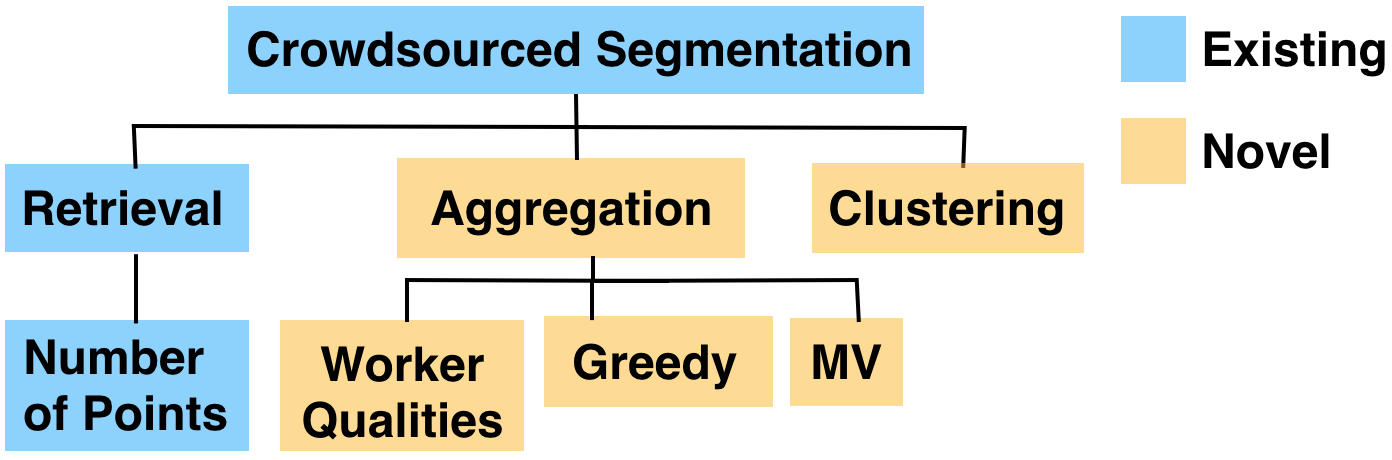
\includegraphics[width=\linewidth]{plots/flowchart.png}
\caption{Flowchart summarizing the classes of existing algorithms for image segmentation (blue) and a novel class of algorithms proposed in this paper (yellow). Majority-vote (MV) is colored both blue and yellow, since a common algorithm in crowdsourcing literature, but have not been extensively applied to crowdsourced image segmentation.}
\vspace{-10pt}
%The crowdsourced approach can be largely classified as retrieval or aggregation-based methods. We further explore hybrid algorithms that makes use of signals that span over multiple categories, described in our technical report.
\label{flowchart}
\end{figure}
%Many large-scale efforts in crowdsourced image segmentation contain little to no information on the quality characterization and evaluation of the collected dataset~\cite{Torralba2010,MartinFTM01,Li2009,Gurari2015}, which indicate the lack of standardized approaches for quality evaluation. 
As shown in Figure \ref{flowchart}, quality evaluation methods for crowdsourced segmentation can be largely classified into two categories:

\stitle{Retrieval-based methods} seek to pick the ``best'' worker segmentation based on some scoring criteria that evaluates the quality of each segmentation, including the use of vision information~\cite{Vittayakorn2011,Russakovsky2015}, expectation-maximization (EM) approaches for bounding box quality estimation~\cite{MDWWelinder2010}, and click-stream behavior \cite{Cabezas2015,Sameki2015,Sorokin2008}.

\stitle{Aggregation-based methods} use multiple worker segmentations to produce a single combined segmentation. %Our paper formulate a novel ``tiles'' approach for aggregation methods that operates on discrete non-overlapping units composed of all worker segmentations overlaid on top of each other. 
\ads{reword a bit to emphasize difference from retrieval; Aggregation-based methods combine multiple worker segmentations to produce a final segmentation, and are not restricted by any single worker segmentation.}
Aggregation-based majority vote have been introduced in Sameki et al. (\citeyear{Sameki2015}) as a way for aggregating expert segmentations to obtain a ground truth segmentation for evaluation purposes. \ads{Not clear how what they did is different from us---important to reword so that novelty of our aggregation methodology (and MV algo in particular) is not questioned.}

%specialized segmentation interfaces or workflows that ensures that the annotations collected are of high quality, including 
Orthogonal methods to improve segmentation quality include periodic verification workflows~\cite{Lin2014,Everingham15}, specialized segmentation interfaces~\cite{Song2018}, and vision-based supervision of crowdsourced segmentation\cite{Russakovsky2015,Gurari2016}. Our paper do not compare against these methods since they are not easily reproducible and could be used for quality improvement on top of any of the algorithms described in this paper.  %Since these policy-based methods are interface-dependent, require expensive expert-drawn ground-truth annotations or vision information, the results are not easily reproducible. In addition, the segmentations collected by the simple click-and-draw interface in many of the large scale segmentation efforts can not be improved with this technique as a post-processing method. Due to the lack of reproducibility, our paper do not compare against these policy-based methods in extensive details.


          \vspace{-7pt}
\section{Error Analysis\label{sec:error}}
\par On collecting and analyzing a number of crowdsourced segmentation (described Section~\ref{dataset}), we found that common worker segmentation errors can be classified into three types: (1) \textbf{Semantic Ambiguity:} workers have differing opinions on whether particular regions belong to an object (Figure~\ref{error_examples} left: annotations around `flower and vase' when `vase' is requested); (2) \textbf{Semantic Mistake:} workers annotate the wrong object entirely (Figure~\ref{error_examples} right: annotations around `turtle' and `monitor' when `computer' is requested.); and (3) \textbf{Boundary Imperfection:} workers make unintentional mistakes while drawing the boundaries, either due to low image resolution, small area of the object, or lack of drawing skills (Figure~\ref{tile_demo} left: imprecision around the `dog' object).
\par Quality evaluation methods in prior work have largely focused on minimizing boundary imperfection issues. So, we first describe our novel aggregation-based algorithms designed to reduce boundary imperfections. Next, in Section~\ref{perspective}, we discuss a preprocessing method eliminates semantic ambiguities and errors, also observed in prior work~\cite{Sorokin2008,Lin2014,Gurari2018}. \changes{We present our experimental evaluation demonstrating in Section~\ref{sec:experiment}.}% and compare them with existing retrieval-based methods in 
%\par %Out of the 46 objects in our dataset, 9 objects suffer from semantic ambiguity, 18 objects from semantic mistakes, and almost all objects suffer from some form of boundary imprecision to varying degrees. 
% \begin{figure*}[ht!]
%     \centering
%     \RawFloats
%     \begin{minipage}[t]{0.65\textwidth}
%     	\vspace{-20pt}
%         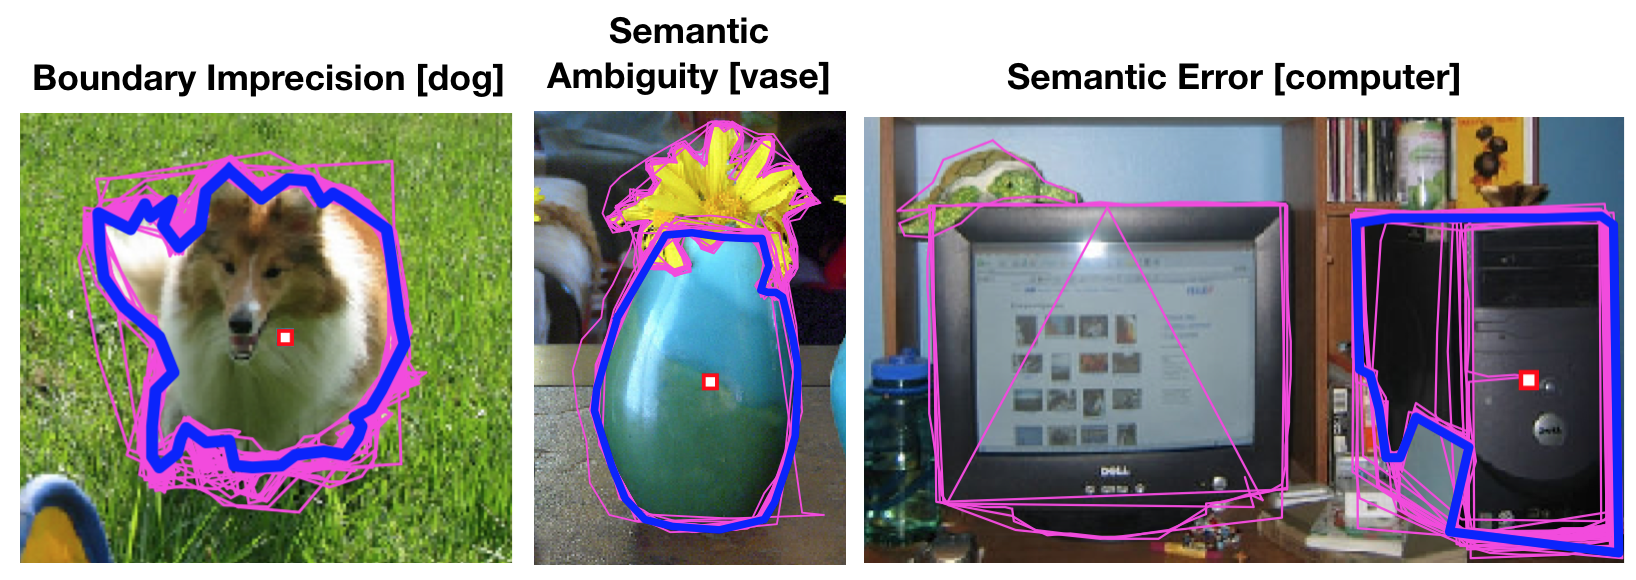
\includegraphics[width=\textwidth]{plots/error_examples.png} % second figure itself
%         \caption{Pink is the segmentation from individual workers. Blue solid line delineates the ground truth. The red boxed pointer indicates the task of interest shown to users.}
%         \vspace{-15pt}
%         \label{error_examples}
%     \end{minipage}
%     \begin{minipage}[t]{0.35\textwidth}
%     	\vspace{-25pt}
%         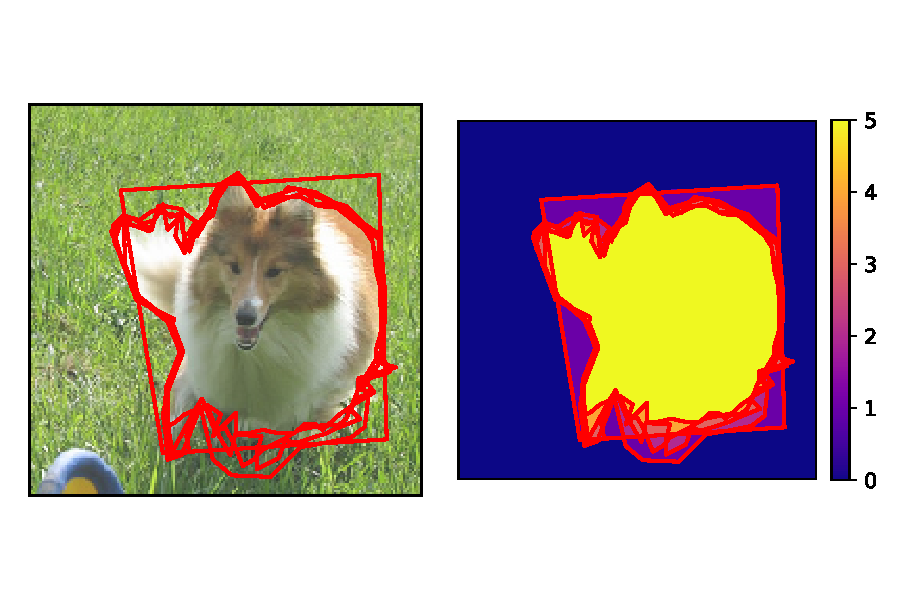
\includegraphics[width=\textwidth]{plots/tile_demo.pdf}
%         \vspace{-35pt}
%         \caption{Segmentation boundaries drawn by five workers in red. Right: Overlaid segmentation creates a masks where the color indicates the number of workers whose segmentation includes the tile region.}
%         \vspace{-20pt}
%         \label{tile_demo}
%     \end{minipage}\hfill
% \end{figure*}
\begin{figure}[h!]
    \centering
    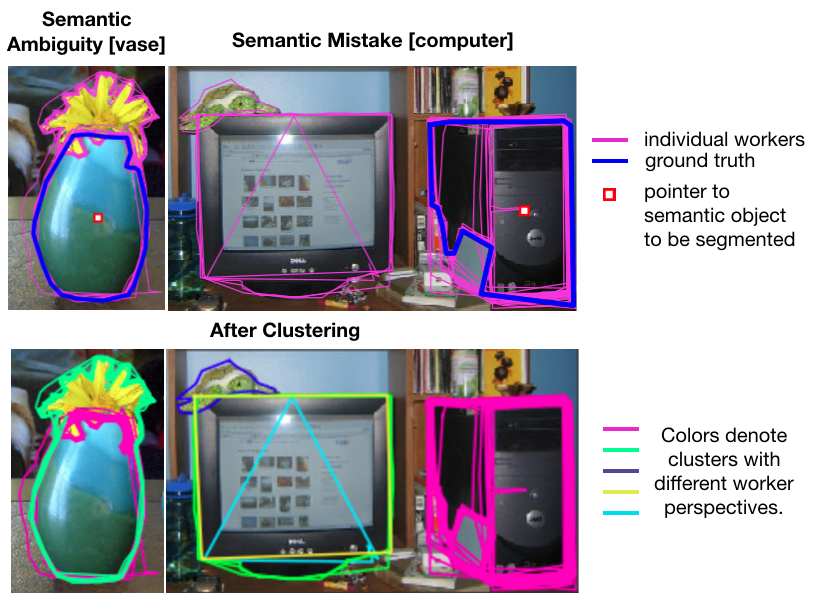
\includegraphics[width=0.9\textwidth]{plots/semantic_error_clust.png}
    \caption{\changes{Top: Examples of semantic ambiguities and mistakes. % where workers display different perspectives on what regions should be included as part of the object. %The pink segmentations are drawn by individual workers. The blue solid line delineates the ground truth. The red boxed pointer is the interface icon indicating the semantic object to be segmented. 
    Bottom: Examples of worker segmentations from different clusters.%, where different colors depict clusters representing different worker perspectives.
    }}
    \label{error_examples}
    \setlength{\abovecaptionskip}{-10pt}
    \setlength{\belowcaptionskip}{-10pt}
\end{figure}
          \section{Precision-focused algorithms}%: Aggregation v.s. Retrieval Comparison}
% \subsection{Retrieval-based methods}
% This class of algorithms tries to identify good and bad workers, and then chooses the best worker segmentation as the output segmentation. In this paper, we look at two different ways of ranking workers and choosing the best worker. First, we use the {\em number of control points}, i.e. number of vertices in a worker's segmentation polygon to rank workers. This is a ranking scheme that~\cite{Vittayakorn2011} showed performs well in practice. Intuitively, workers that have used a larger number of points are likely to have been more precise, and provided a more complex and accurate segmentation. Other heuristic ranking scheme is described in more detail in our technical report~\cite{segmentation-tr}.
\begin{figure}[h!]
\vspace{-10pt}
\centering
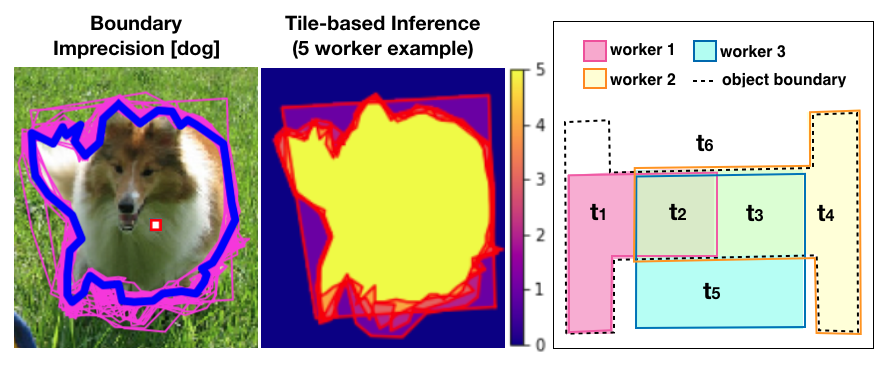
\includegraphics[width=0.8\textwidth]{plots/precision_issue_tile_example.png}
\caption{Left: Pink boundaries shows worker segmentations and blue delineates the ground truth. Right: Segmentation boundaries drawn by five workers shown in red. Overlaid segmentation creates a masks where the color indicates the number of workers who voted for the tile region.}
\label{tile_demo}
\end{figure}
\vspace{-10pt}
At the heart of our aggregation techniques is the ``tile'' data representation, where we logically overlay all workers' segmentations on top of each other, as illustrated in Figure \ref{tile_demo} right, to create non-overlapping discrete tile units. The intuition here is that by splitting the image into tiles, we get finer granularity information than by looking at complete segmentations. This also allows us to aggregate data from multiple workers rather than having to choose a single worker bounding box---enabling the opportunity to choose partial segmentations by fixing one worker's errors via the help from another worker's segmentation. Now, we will describe several algorithms for picking a good set of tiles.

\stitle{Aggregation: Majority Vote Aggregation (MV)} 
\par \noindent Include tiles in the output segmentation if and only if the tile is covered by at least 50\% of all worker segmentations.

\stitle{Aggregation: Expectation-Maximization (EM)}
\par \noindent Unlike MV, which assumes that all workers performs uniformly, EM approaches use worker quality models to infer the likelihood that a tile is part of the ground truth segmentation. The EM algorithm simultaneously estimate both worker qualities and tile likelihoods as hidden variables. Details of the formal derivation and three worker quality models that we have developed can be found in our technical report.

\stitle{Aggregation: Greedy Tile Picking (greedy)} 
\par \noindent Using tile probabilities from EM to estimate intersection area between ground truth and tile, then greedily pick tiles with the largest intersection area ratio until Jaccard score begins to decrease (effectively picking the largest and most probable tiles that should be included first). The Jaccard score is computed between the merged output from the selected set of tiles and MV segmentation.

\stitle{Retrieval: Number of Control Points (num pts)}
\par \noindent Pick the worker segmentation with the largest number of control points around the segmentation boundary (i.e. most precise drawing) as the output segmentation.
          %!TEX root = main.tex
\section{Perspective Resolution in Crowdsourced Image Segmentation}
\subsection{Worker Clustering}
Our clustering-based approach is based on the intuition that workers with similar perspectives  will have segmentations that are closer to each other, while workers with different perspectives from each other will have segmentations that differ from each other. We capture the similarity between a pair of workers by computing the Jaccard score between their segmentations and perform {\em spectral clustering} to separate workers into clusters. Figure \ref{cluster_example} illustrates how spectral clustering is capable of dividing the worker responses into clusters with meaningful semantic associations, reflecting the crowd's diversity of perspectives in completing same task.
    \begin{figure}[ht!]
      \centering
      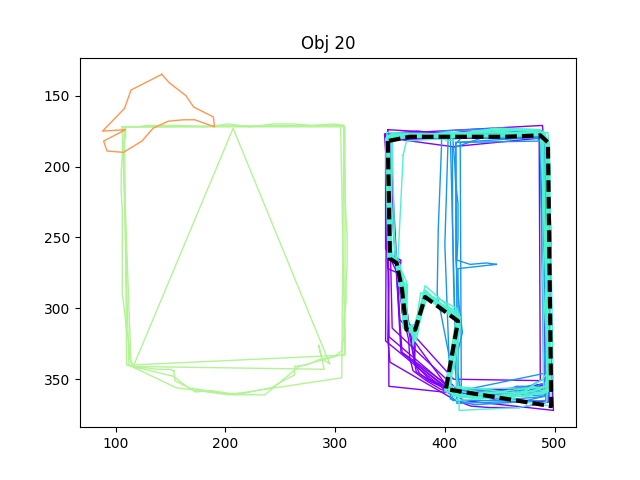
\includegraphics[width=\textwidth]{plots/20.png}
      \caption{Example image showing clustering performed on the same object from Figure \ref{error_examples}.}
      \label{cluster_example}
    \end{figure}
\par Clustering results can also be used as a preprocessing step to any of the quality evaluation algorithms by keeping only the segmentations that belong to the largest cluster, which is typically free of any semantic errors. As shown in Table~\ref{statsTable}, on average, clustering generally results in an increase the resulting algorithmic performance. Since the ground-truth supervised variants are already free of semantic ambiguity and errors, there is minimal improvement resulting from clustering. %In particular, we see a greater improvement with clustering preprocessing for algorithms that are not very robust in resolving semantic errors or ambiguity, such as for the \texttt{num pts} retrieval algorithm, than compared to the aggregation-based methods. 
\par Clustering offers an additional benefit of preserving worker's semantic intentions in the case where there are multiple instances of different errors. For example, in Figure \ref{cluster_example}, the mistakened clusters included semantic concepts ``monitor'' and ``turtle''. While these are considered \textit{bad} annotations for this particular task, this cluster of annotation can provide more data for another semantic segmentation task ``monitor''. A potential direction of future work includes adding an additional crowdsourcing task for semantic labelling of clusters (which is cheaper and more accurate than segmentation) to enable reuse of annotations across objects and lower the cost of data collection. 
          %!TEX root = main.tex
\section{Experimental Evaluation\label{sec:experiment}}

\stitle{Dataset Description\label{dataset}}
\par \noindent We collected crowdsourced segmentations from Amazon Mechanical Turk; each HIT consisted of one segmentation task for a specific pre-labeled object in an image. There were a total of 46 objects in 9 images from the MSCOCO dataset~\cite{Lin2014} segmented by 40 different workers each, resulting in a total of 1840 segmentations. Each task contained a keyword for the object and a pointer indicating the object to be segmented. Two of the authors generated the ground truth segmentations by carefully segmenting the objects using the same task and interface. %segmented the objects using our own segmentation interface and use the generated segmentations as ground truth data.%\agp{How did you get GT?} \dor{I just annotated very carefully to draw around the object as the GT, could not use the COCO annotations because of the semantic segmentation they used were different, so there ends up being a lot of semantic ambiguity. We should probably not get into the details here.}%These tasks represent a diverse set of task difficulty (different levels of clutteredness, occlusion, lighting) and levels of task ambiguity. 
\techreport{\par A sub-sampled dataset was created from the full dataset to determine the efficacy of these algorithms on varying number of worker responses. Every object was randomly sampled worker with replacement. For small worker samples, we average our results over larger number of batches than for large worker samples (which have lower variance, since the sample size is close to the original data size).}

\stitle{Evaluation Metrics}
\par \noindent Evaluation metrics used in our experiments measure how well the final segmentation (S) produced by these algorithms compare against ground truth (GT). The most common evaluation metrics used in the literature are area-based methods  that take into account the intersection area, $IA=area(S\cap GT)$, or union area, $UA=area(S\cup GT)$ between the worker and ground truth segmentations, including %. Specifically, we use
    $\text{Precision (P)} = \frac{IA(S)}{area(S)}$, 
    $\text{Recall (R)} = \frac{IA(S)}{area(GT)}$, and 
    $\text{Jaccard (J)} = \frac{UA(S)}{IA(S)}$.
    %metrics to evaluate our algorithms.

\stitle{Experiment 1: Aggregation-based methods perform significantly better than retrieval-based methods}
\begin{figure}[h!]
   \centering
   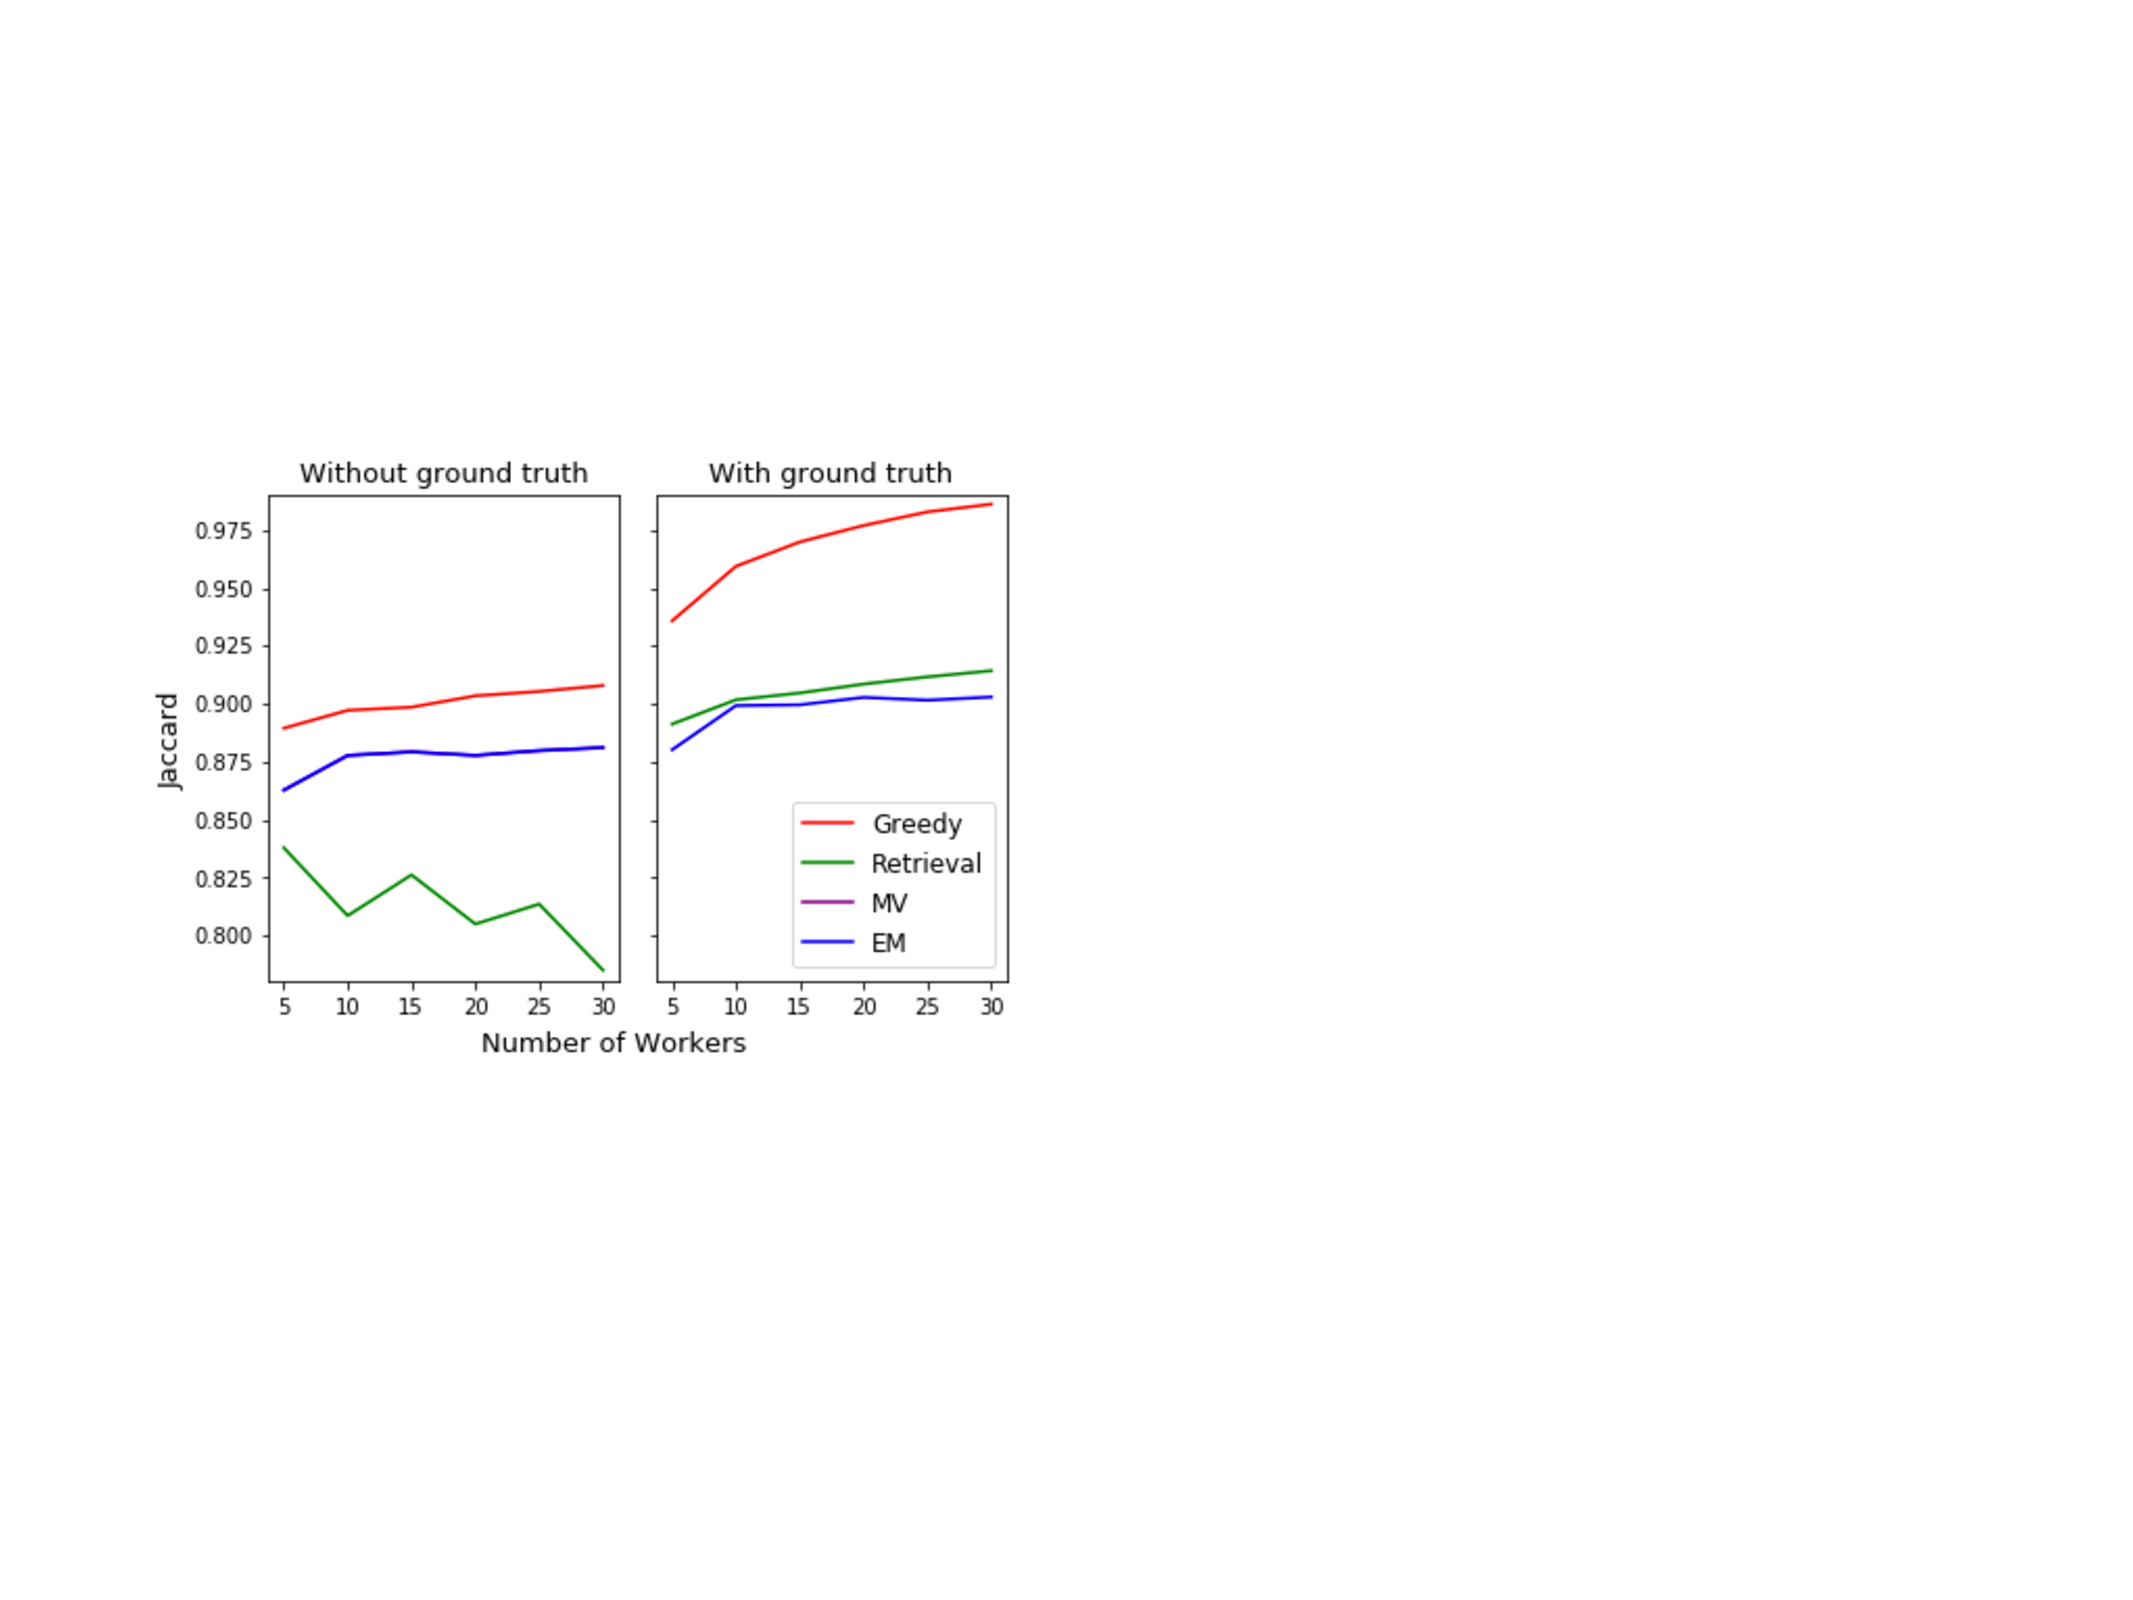
\includegraphics[trim={0 1pt 4pt 0},clip,width=0.8\linewidth]{plots/Retrieval_vs_Aggregation.pdf}
   \caption{Performance of the original algorithms that do not make use of ground truth information (Left) and ones that do (Right). MV and EM results are so close that they overlay on each other.} %\agp{Explain setup for this. How did you generate this?} \dor{not sure what aditya means?}}%Performance comparison between best-performing retrieval and aggregation-based methods. 
   \label{retrieval_vs_aggregation}   
   \vspace{-12pt}
   \setlength{\abovecaptionskip}{-30pt}
   \setlength{\belowcaptionskip}{-23pt}
\end{figure} 
\npar In Figure~\ref{retrieval_vs_aggregation}, we vary the number of worker segmentations along the x-axis and plot the average Jaccard score on the y-axis across different worker samples of a given size across different algorithms. Figure~\ref{retrieval_vs_aggregation} (left) shows that the performance of aggregation-based algorithms (greedy, EM) exceeds the best-achievable through existing retrieval-based method (Retrieval). Then, in Figure \ref{retrieval_vs_aggregation} (right), we estimate the upper-bound performance of each algorithm by assuming that the `full information' based on ground truth was given to the algorithm. For greedy, the algorithm is aware of all the actual tile overlap and non-overlap areas against ground truth, and does not need to approximate these values. For EM, we consider the performance of the algorithm if the true worker quality parameter values (under our worker quality model) are known. For retrieval, the full information version directly picks the worker with the highest Jaccard similarity with respect to the ground truth segmentation. By making use of ground truth information (Figure~\ref{retrieval_vs_aggregation} right), the best aggregation-based algorithm can achieve a close-to-perfect average Jaccard score of 0.98 as an upper bound, far exceeding the results achievable by any single `best' worker (J=0.91). This result demonstrates that aggregation-based methods are able to achieve better performance by performing inference at the tile granularity, which is guaranteed to be finer grained than any individual worker segmentation. 

\stitle{The performance of aggregation-based methods scale well as more worker segmentations are added.}
\par \noindent Intuitively, larger numbers of worker segmentations result in finer granularity tiles for the aggregation-based methods. The first row in Table~\ref{statsTable} lists the average percentage change in Jaccard between 5-workers and 30-workers samples, demonstrating a monotonically increasing relationship between number of worker segmentations used and the performance. However, retrieval-based methods do not benefit from more segmentations.

\stitle{Experiment 2: Clustering as preprocessing improves algorithmic performance.}
\par \noindent The average percentage change between the no clustering and clustering results is shown in Table~\ref{statsTable}. Clustering generally results in an accuracy increase. Since the `full information' variants are already free of semantic ambiguity and errors, clustering does not assist with further improvement. %In particular, we see a greater improvement with clustering preprocessing for algorithms that are not very robust in resolving semantic errors or ambiguity, such as for the \texttt{num pts} retrieval algorithm, than compared to the aggregation-based methods. 
%\agp{Weird, this is experiment 2. Divide this up into two parts. (Right now it seems as if all findings are from Fig 4, so this comes as a surprise.)}\dor{should we divide table~\ref{statsTable} into two separate tables?}
\begin{table}[h!]
   \small
     \setlength\tabcolsep{1.5pt}
      \begin{tabular}{l|l|l|l|l|l|l}
         & \multicolumn{2}{c|}{Retrieval-based} & \multicolumn{4}{l}{Aggregation-based} \\ \hline
      Algorithm         & num pts         & worker*        & MV    & EM    & greedy  & greedy*  \\ \hline
      Worker Scaling    & -6.30           & 2.58               & 1.63  & 1.64  & 2.16    & 5.59         \\ \hline
      Clustering Effect & 5.92            & -0.02              & 2.05  & 1.38  & 5.55    & -0.06       
      \end{tabular}
      \caption{Percentage change due to worker scaling and clustering. Algorithms with * makes use of ground truth information.}
      \label{statsTable}
\end{table}
          \section{Experimental Results\label{sec:experiment}}
\subsection{Aggregation-based methods perform significantly better than retrieval-based methods (no clustering)}
\begin{figure}[h!]
   \centering
   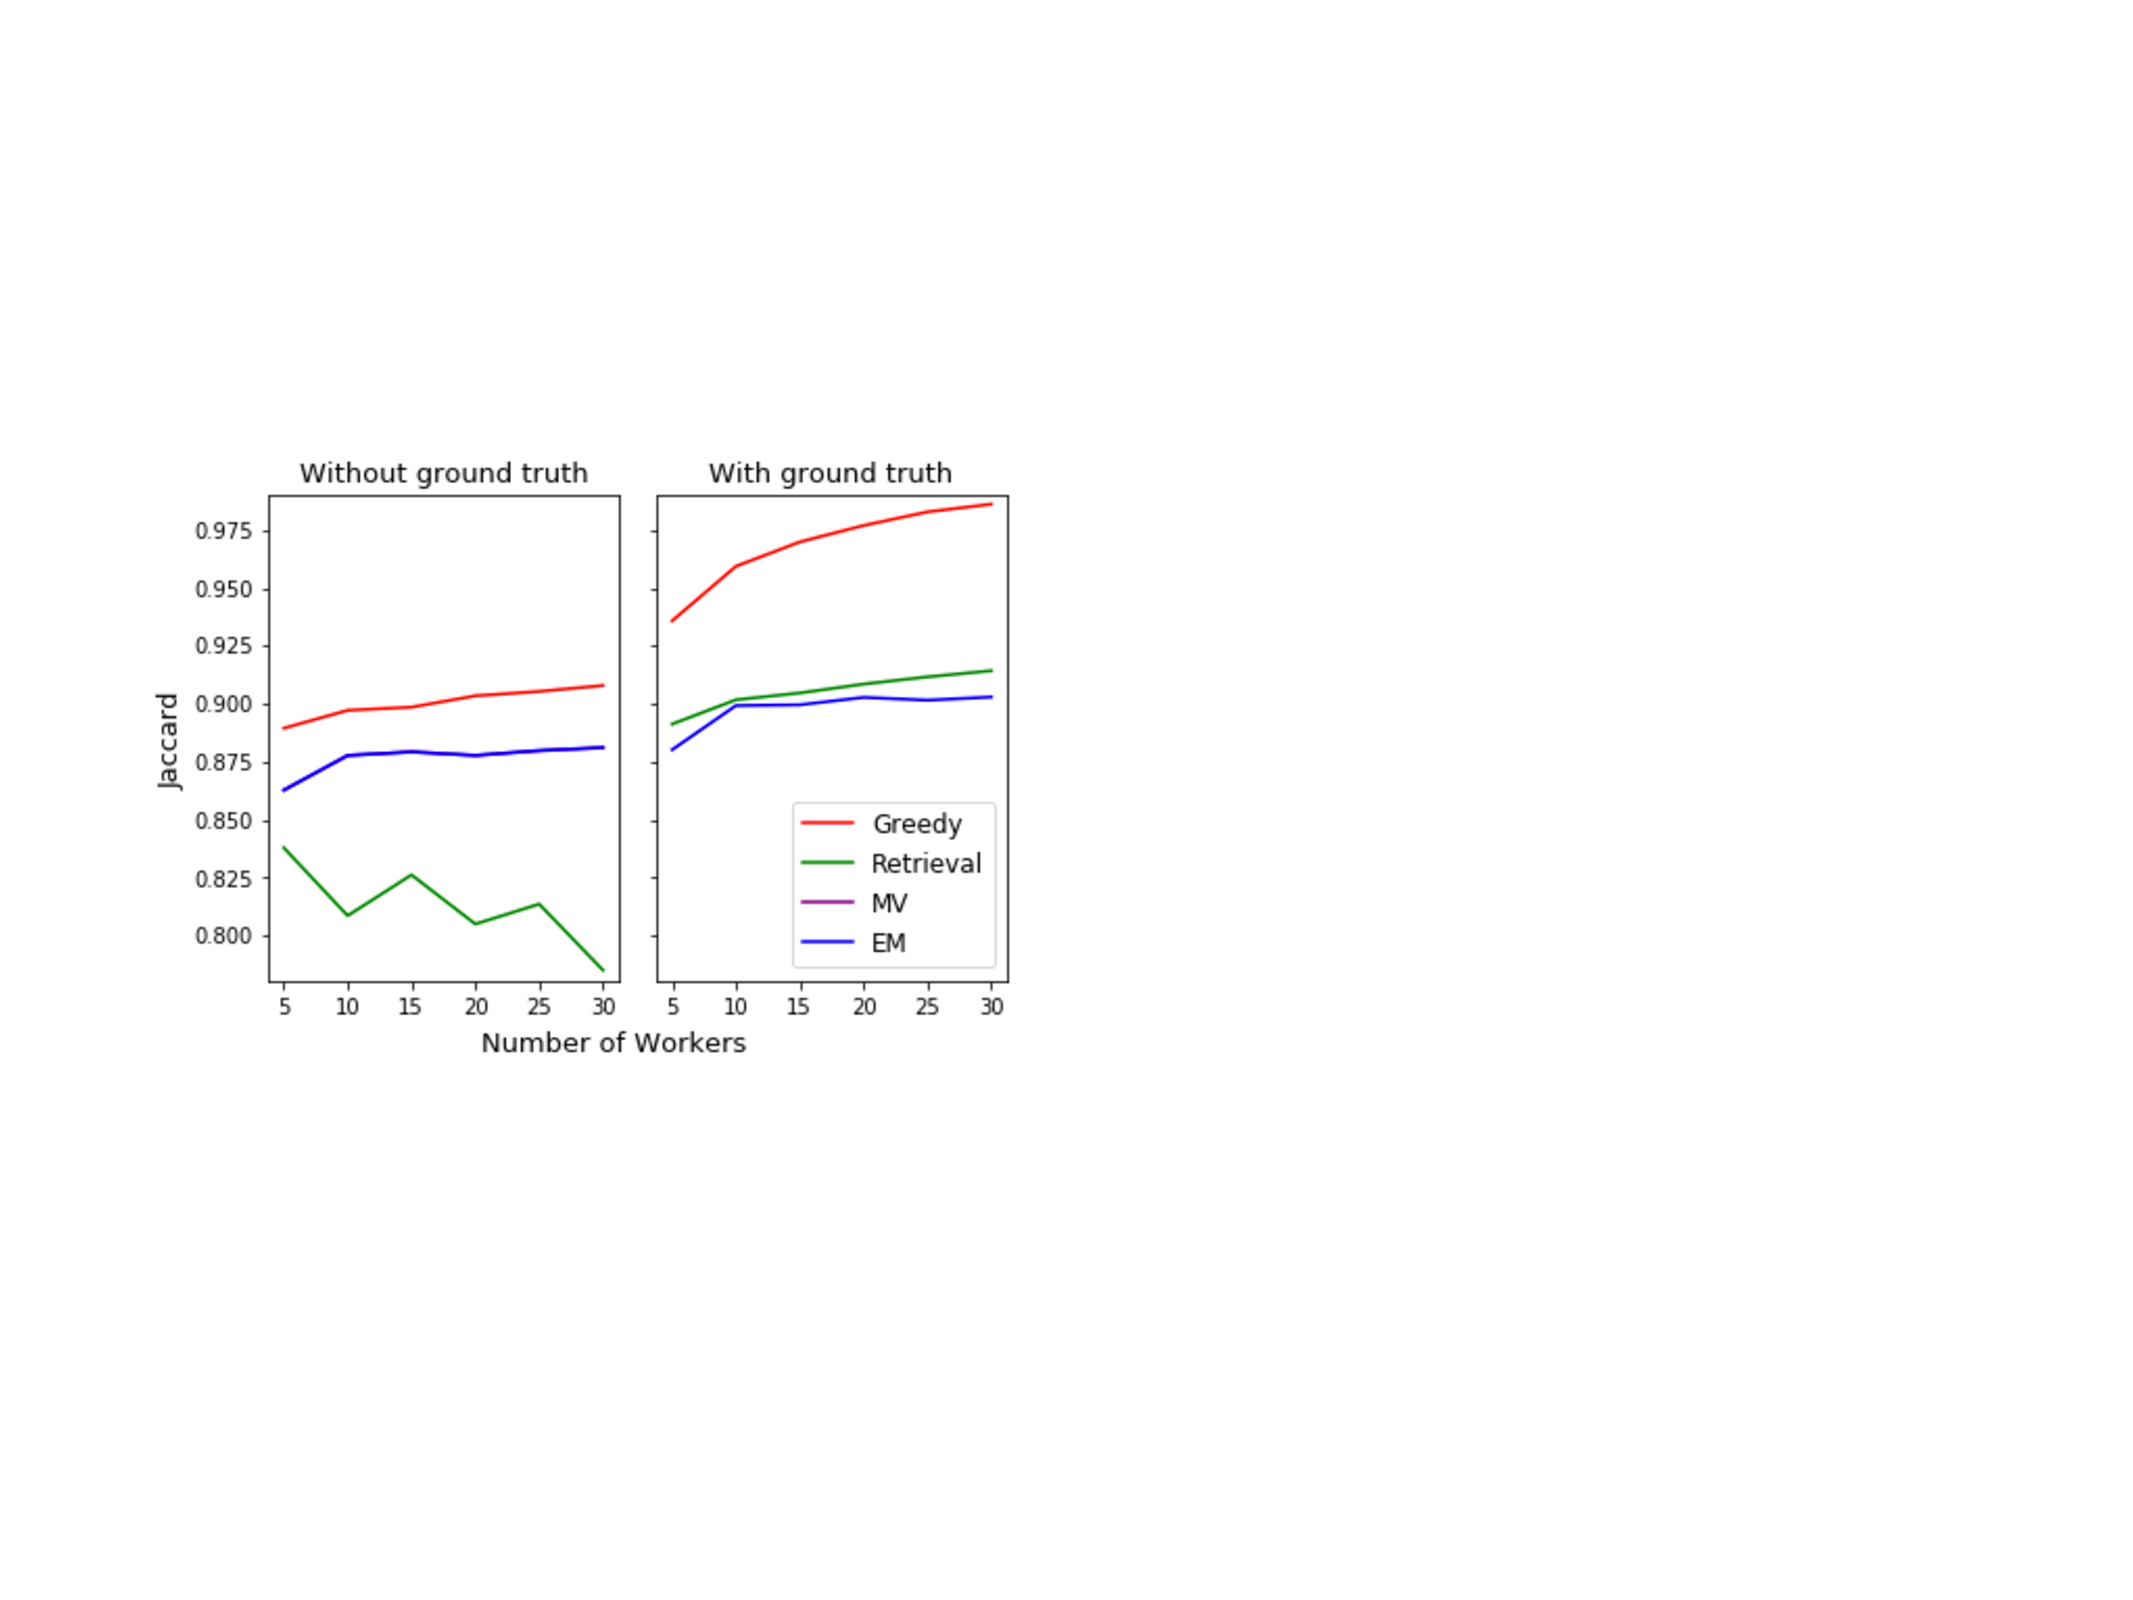
\includegraphics[trim={0 1pt 4pt 0},clip,width=0.8\linewidth]{plots/Retrieval_vs_Aggregation.pdf}
   \caption{Performance of the original algorithms that do not make use of ground truth information (Left) and ones that do (Right). MV and EM results are so close that they overlay on each other.} 
   \label{retrieval_vs_aggregation}   
\end{figure} 
\npar In Figure~\ref{retrieval_vs_aggregation}, we vary the number of worker segmentations along the x-axis and plot the average Jaccard score on the y-axis across different worker samples of a given size across different algorithms. Figure~\ref{retrieval_vs_aggregation} (left) shows that the performance of aggregation-based algorithms (greedy, EM) exceeds the best-achievable through existing retrieval-based method (Retrieval). Then, in Figure \ref{retrieval_vs_aggregation} (right), we estimate the upper-bound performance of each algorithm by assuming that the `full information' based on ground truth was given to the algorithm. For greedy, the algorithm is aware of all the actual tile overlap and non-overlap areas against ground truth, and does not need to approximate these values. For EM, we consider the performance of the algorithm if the true worker quality parameter values (under our worker quality model) are known. For retrieval, the full information version directly picks the worker with the highest Jaccard similarity with respect to the ground truth segmentation. By making use of ground truth information (Figure~\ref{retrieval_vs_aggregation} right), the best aggregation-based algorithm can achieve a close-to-perfect average Jaccard score of 0.98 as an upper bound, far exceeding the results achievable by any single `best' worker (J=0.91). This result demonstrates that aggregation-based methods are able to achieve better performance by performing inference at the tile granularity, which is guaranteed to be finer grained than any individual worker segmentation. 

\subsection{The performance of aggregation-based methods scale well as more worker segmentations are added.}
\par \noindent Intuitively, larger numbers of worker segmentations result in finer granularity tiles for the aggregation-based methods. The first row in Table~\ref{statsTable} lists the average percentage change in Jaccard between 5-workers and 30-workers samples, demonstrating a monotonically increasing relationship between number of worker segmentations used and the performance. However, retrieval-based methods do not benefit from more segmentations.

\subsection{Clustering as preprocessing improves algorithmic performance.}
\par \noindent The average percentage change between the no clustering and clustering results is shown in Table~\ref{statsTable}. Clustering generally results in an accuracy increase. Since the `full information' variants are already free of semantic ambiguity and errors, clustering does not assist with further improvement. %In particular, we see a greater improvement with clustering preprocessing for algorithms that are not very robust in resolving semantic errors or ambiguity, such as for the \texttt{num pts} retrieval algorithm, than compared to the aggregation-based methods. 
\begin{table}[h!]
     \small
     % \setlength\tabcolsep{1.5pt}
     \scalebox{0.85}{
      \begin{tabular}{l|l|l|l|l|l|l|l}
      & \multicolumn{3}{c|}{Retrieval-based} & \multicolumn{4}{l}{Aggregation-based} \\ \hline
      Algorithm       & num pts     & worker    & worker*    & MV     & EM     & greedy   & greedy*   \\ \hline
      Worker Scaling    & -6.30       & -0.25     & 2.58       & 1.63   & 1.64   & 2.16     & 5.59      \\ \hline
      Clustering Effect & 5.92        & 4.00      & -0.02      & 2.05   & 1.38   & 5.55     & -0.06    
      \end{tabular}
      }
      \caption{Jaccard percentage change due to worker scaling and clustering. Algorithms with * makes use of ground truth information.}
      \label{statsTable} 
\end{table}
\par The clustering preprocessing step can significantly improve performance of algorithms that are not very robust to segmentations with semantic errors or ambiguities, such as the heuristic-based number of points approach. When examining the gap of increase with and without clustering in Figure \ref{cluster_effect}, we find that aggregation-based methods performs better than retrieval-methods exhibits a smaller gap between the performances. This effect is due to aggregation-based method's higher performance in the no cluster case, indicating that it is able to capture some of the semantic ambiguities and errors in the dataset.
\begin{figure}[ht!]
      \centering
      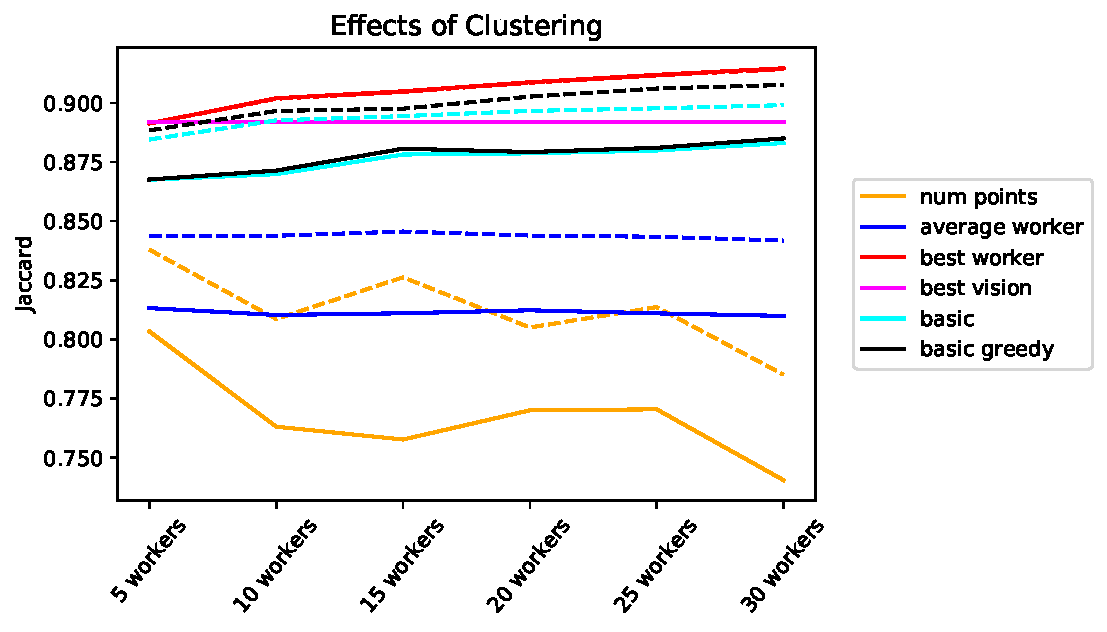
\includegraphics[width=\linewidth]{plots/Effects_of_clustering.pdf}
      \caption{Performance comparisons between averaging over experiments with clustering as a preprocessing step (dotted) and the unclustered results (solid) for different algorithms.}
      \label{cluster_effect}
\end{figure}
\subsection{How well does the inferred worker qualities predict individual worker performance?}
    \stitle{Correlation of worker qualities against performance}
     To further investigate how the EM models are performing, we looked at whether the model-inferred worker qualities is indicative of the actual quality of a segmentation. We performed linear fitting independently for each sample-objects and computed the $R^2$ statistics to determine whether worker qualities can accurately predict precision, recall, and Jaccard scores. Visual inspection of the basic worker quality model fitting showed that for objects that suffered from type two errors (semantic ambiguity), the single-parameter worker quality was unable to capture the overbounding behavior, which lead to a low precision and Jaccard. The results are listed in Table \ref{correlation} to highlight how our advanced worker qualities were able to better capture these scenarios. The clustering preprocessing was not performed for the values in Table \ref{correlation} to demonstrate the sole effect of the EM algorithm. Nevertheless, our clustered results also show a similar trend, with an average of $R^2$=0.88 and 0.89 for the GT and GTLSA models across all objects respectively. We also find that in general the linear fit improves as the number of data points increases, which indicates consistency in the fitted model.
    \begin{table}[ht!]
      \small
      \begin{tabular}{ccccccc}
        \hline
           N &   basic &   GT &   GTLSA &   isobasic &   isoGT &   isoGTLSA \\
        \hline
              5 &      0.601 &   0.907 &      0.901 &       0.576 &    0.907 &       0.904 \\
            10 &      0.632 &   0.895 &      0.899 &       0.633 &    0.895 &       0.898 \\
            15 &      0.622 &   0.897 &      0.898 &       0.622 &    0.897 &       0.897 \\
            20 &      0.636 &   0.894 &      0.899 &       0.637 &    0.894 &       0.898 \\
            25 &      0.66  &   0.901 &      0.905 &       0.661 &    0.901 &       0.904 \\
            30 &      0.673 &   0.907 &      \cellcolor{blue!25}0.914 &       0.676 &    0.907 &       \cellcolor{blue!25}0.913 \\
        \hline
      \end{tabular}
        \caption{Linear correlation of worker qualities against ground truth performance for different quality models across different number of workers (N). The lower worker samples exhibit lower $R^2$ due to the variance from smaller number of datapoints for each independent fit. }
        \label{correlation}
    \end{table}
    % \subsubsection{EM performance with different worker quality models}
    %   - why is iso cases not performing as well
    \stitle{Best worker quality retrieval}
    One application of worker qualities is that it could be used as an annotation scoring function for retrieving the best quality worker segmentation. We explore this approach by training a linear regression model for every sample-object and use the worker qualities to predict the precision, recall, and Jaccard of individual worker annotations against ground truth. Then, we query the model with the inferred worker quality and retrieve the worker with the best predicted Jaccard. 
    \par The reason why a linear regression model was chosen rather than simply sorting the worker qualities and picking the best is that sorting based on multiple worker qualities (precision, recall, Jaccard) effectively applies equal weighting to all quality attributes, whereas our advanced models are specifically designed to capture cases of false-positives and false-negatives that can yield drastically different recall and precision values. We have tested that the linear regression model performs better on this task that simple sorting is capable of learning the weights that helps it make better predictions. As shown in Table~\ref{bigtable}, the performance of worker-quality based retrieval is comparable the performance other aggregation-based methods. We find that amongst the different worker quality models, advanced worker quality models perform the best, agreeing with our intuition regarding correlation results observed in Table~\ref{correlation}.
    \begin{table}[ht!]
    \small
    \setlength\tabcolsep{3pt}
    \begin{tabular}{lrrrrrr}
      \hline
       algo/N                  &     5 &    10 &    15 &    20 &    25 &    30 \\
      \hline
       num points           & 0.838 & 0.809 & 0.826 & 0.805 & 0.814 & 0.785 \\
       best worker          & 0.891 & 0.902 & 0.905 & 0.909 & 0.912 & 0.914 \\
       \hline
       MV                   & 0.885 & 0.893 & 0.894 & 0.897 & 0.898 & 0.899 \\
       EM[basic]           & 0.884 & 0.893 & 0.894 & 0.897 & 0.898 & 0.899 \\
       EM[GT]              & 0.885 & 0.893 & 0.894 & 0.897 & 0.898 & 0.899 \\
       EM[GTLSA]           & 0.871 & 0.892 & 0.891 & 0.896 & 0.897 & \cellcolor{blue!25} 0.899 \\
       greedy               & 0.888 & 0.896 & 0.896 & 0.902 & 0.905 & 0.906 \\
       wqr[basic]          & 0.878 & 0.877 & 0.877 & 0.877 & 0.878 & 0.878 \\
       wqr[GT]             & 0.884 & 0.885 & 0.885 & 0.885 & 0.887 & 0.887 \\
       wqr[GTLSA]          & 0.874 & 0.881 & 0.883 & 0.885 & 0.886 & \cellcolor{blue!25} 0.887 \\
      \hline
    \end{tabular}
    \caption{Summary of average performance across workers with clustering applied as preprocessing in all algorithms across different number of workers (N). wqr is the abbreviation for best worker quality retrieval methods.}
    \label{bigtable}
    \end{table}
          \section{Conclusion}
In this paper, we perform an extensive study of several image segmentation algorithms spanning semi-supervised vision approaches, crowdsourced retrieval approaches, and novel crowdsourced aggregation approaches. We identified three different types of errors that workers typically make on segmentation tasks, some caused by differing perspectives, and developed a clustering-based method to filter out workers that are making semantic errors. We demonstrate the strength of our worker clustering algorithm as well as the aggregation-based segmentation algorithms through extensive experiments in 1) its ability to improve as more worker segmentations are collected and 2) yield better performance than retrieval-based methods. We also found that while majority vote is a fairly simple algorithm, it performs nearly as well as the advanced EM and greedy inference approaches. Our code is open source and available for researchers to benchmark and compare techniques. Our work represents a first step in understanding and comparing the different types of algorithms available for image segmentation tasks. It opens a number of exciting directions for exploration, for instance: (a) Studying the effect of task difficulty, or worker qualities across different, objects, and (b) Designing better hybrid algorithms that combine the different types of algorithms described in this paper.

% \balance  
\bibliographystyle{ACM-Reference-Format}
\bibliography{reference}
\end{document}
